\documentclass[20pt]{extarticle}
\usepackage[paperwidth=594mm,paperheight=841mm,margin=16mm]{geometry}
\usepackage{multicol}
\usepackage{graphicx}
\usepackage{amsmath}
\usepackage{booktabs}
\usepackage{xcolor}
\usepackage{tikz}
\usetikzlibrary{positioning}
\usepackage{enumitem}
\usepackage{tcolorbox}
\usepackage{helvet}
\usepackage[hidelinks]{hyperref}
\renewcommand{\familydefault}{\sfdefault}

\definecolor{navy}{HTML}{0B2545}
\definecolor{teal}{HTML}{13A89E}
\definecolor{amber}{HTML}{F2A541}
\definecolor{lightgrey}{HTML}{F4F6F8}

\setlength{\columnsep}{9mm}
\setlength{\columnseprule}{0.4pt}
\setlength{\parindent}{0pt}
\setlength{\parskip}{2.5mm}
\pagestyle{empty}

\newcommand{\heading}[1]{%
  \vspace{3mm}%
  {\color{navy}\fontsize{30}{34}\selectfont\bfseries #1}\\[-1.5mm]%
  {\color{teal}\rule{\linewidth}{0.9mm}}\par\vspace{1.5mm}%
}

\begin{document}

\begin{center}
{\color{navy}\fontsize{68}{76}\selectfont\bfseries Machine-Learning Wireless\\[1mm]
Intrusion Detection System}\\[4mm]
{\color{teal}\fontsize{34}{40}\selectfont\bfseries Detecting 802.11 Deauthentication Floods\\[1mm]
with a Random Forest}\\[4mm]
{\fontsize{26}{30}\selectfont Ted Kamau}\\[2mm]
{\fontsize{20}{24}\selectfont WIDS/WIPS Assignment, November 2026}
\end{center}

\vspace{-2mm}
{\color{navy}\rule{\linewidth}{2.2mm}}
\vspace{2mm}

\begin{tcolorbox}[colback=amber!18,colframe=amber,boxrule=1.2pt,arc=2mm,
  left=6mm,right=6mm,top=3mm,bottom=3mm]
{\fontsize{24}{28}\selectfont\bfseries A Random Forest looks at each MAC address every second and flags deauthentication floods. On held-out traffic it got 100\% accuracy and named the MAC that caused the flood.}
\end{tcolorbox}

\begin{multicols}{3}

\heading{The problem}
Deauthentication frames are management frames, and many networks do not
protect them. An attacker can spoof them and kick clients off the network.
That is a denial of service, and it can also help an evil twin attack. A
\textbf{WIDS} detects this and raises an alert. A WIPS would also block it.
I built the WIDS.

\heading{Dataset}
I used one capture from the public \textbf{WPA3 Attacks Dataset} (Mendeley
Data, CC BY 4.0): the deauthentication attack capture.

\begin{itemize}[leftmargin=5mm,itemsep=1mm,topsep=1mm]
  \item 916 s, 722,606 frames
  \item 515,384 normal frames
  \item 207,222 deauth-labelled frames
  \item 370 s flood; peak over 1,300 deauth/s
  \item Isolated WPA3 testbed built by the dataset authors
  \item No new traffic captured or generated
\end{itemize}

{\fontsize{17}{21}\selectfont
\textbf{Citation:} Halbouni, Ong \& Leow (2026), \emph{WPA3 Attacks Dataset},
DOI 10.17632/cxx5t5nw7z.3, CC BY 4.0.\par}

\heading{Features}
I made one row per \textbf{transmitter MAC per second}: 2,692 rows, 235 MACs
and 22 features. The model does not get the MAC address or the timestamp.

\begin{center}
\fontsize{17}{21}\selectfont
\begin{tabular}{@{}p{0.44\linewidth}p{0.46\linewidth}@{}}
\toprule
\textbf{Feature} & \textbf{Why it matters} \\
\midrule
deauth count / ratio & Direct flood signal \\
frames per second & Flood volume \\
frame-type counts & Management vs data mix \\
mean / std RSSI & Transmitter proximity \\
unique destinations & Broadcast / spoof pattern \\
retry ratio & Channel stress \\
reason-code count & Deauth/disassoc variety \\
\bottomrule
\end{tabular}
\end{center}

\heading{System architecture}
\begin{center}
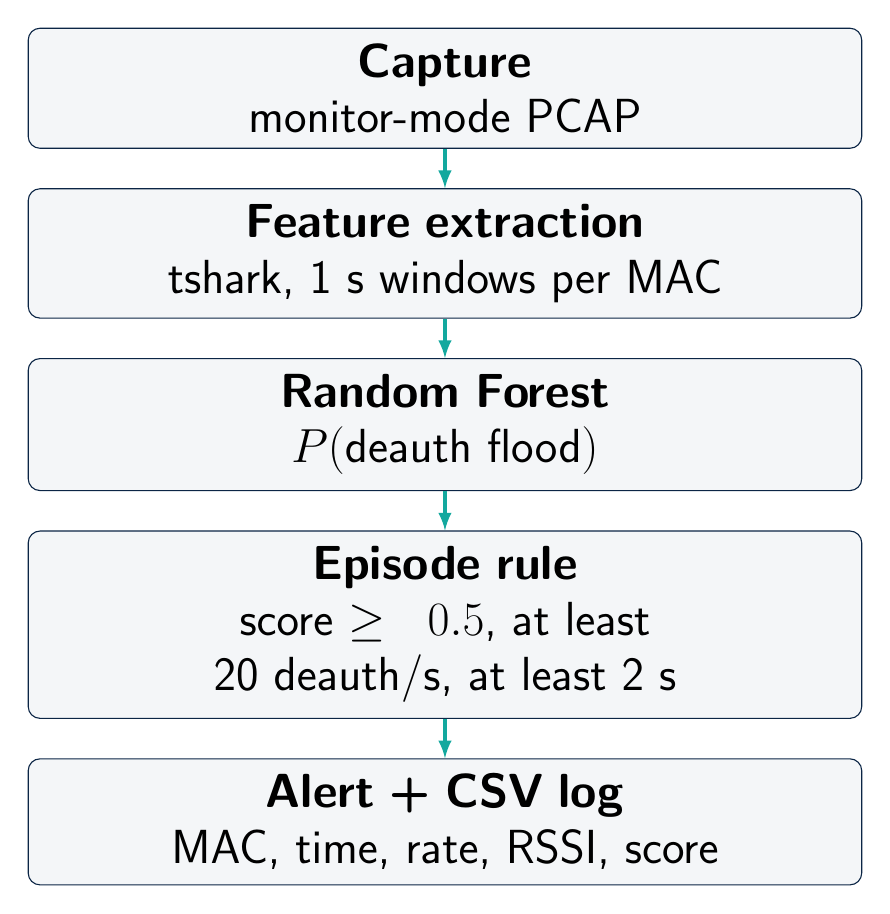
\begin{tikzpicture}[
  box/.style={draw=navy,fill=lightgrey,rounded corners=1.5mm,align=center,
    font=\fontsize{17}{20}\selectfont,text width=0.84\linewidth,
    minimum height=13mm,inner sep=2mm},
  arr/.style={-latex,thick,teal,line width=1.2pt}
]
\node[box] (cap) {\textbf{Capture}\\monitor-mode PCAP};
\node[box,below=5mm of cap] (feat) {\textbf{Feature extraction}\\tshark, 1 s windows per MAC};
\node[box,below=5mm of feat] (ml) {\textbf{Random Forest}\\$P(\text{deauth flood})$};
\node[box,below=5mm of ml] (rule) {\textbf{Episode rule}\\score $\ge 0.5$, at least 20 deauth/s, at least 2 s};
\node[box,below=5mm of rule] (alert) {\textbf{Alert + CSV log}\\MAC, time, rate, RSSI, score};
\draw[arr] (cap) -- (feat);
\draw[arr] (feat) -- (ml);
\draw[arr] (ml) -- (rule);
\draw[arr] (rule) -- (alert);
\end{tikzpicture}
\end{center}

\columnbreak

\heading{Machine learning}
\begin{itemize}[leftmargin=5mm,itemsep=1mm,topsep=1mm]
  \item Random Forest: 300 trees, depth 10, balanced class weights.
  \item Baseline: Decision Tree, depth 6.
  \item Median imputation for missing RSSI.
  \item \textbf{Time-based split:} earlier traffic for training, later traffic held out. No random window leakage.
  \item 1,973 training windows and 719 test windows (607 normal, 112 attack).
\end{itemize}

\heading{Results}
\begin{center}
\fontsize{18}{22}\selectfont
\begin{tabular}{@{}lrr@{}}
\toprule
\textbf{Metric} & \textbf{Random Forest} & \textbf{Decision Tree} \\
\midrule
Accuracy  & 100.0\% & 100.0\% \\
Precision & 100.0\% & 100.0\% \\
Recall    & 100.0\% & 100.0\% \\
F1        & 100.0\% & 100.0\% \\
\bottomrule
\end{tabular}
\end{center}

\textbf{Confusion matrix (RF):} TN 607, FP 0, FN 0, TP 112.

The flood is easy to separate. Normal traffic still has 436 windows with some
deauth frames (up to 64/s), but the attack sends hundreds to over 1,300/s.
The lowest attack score was 0.85 and the highest normal score was 0.28.

\begin{center}
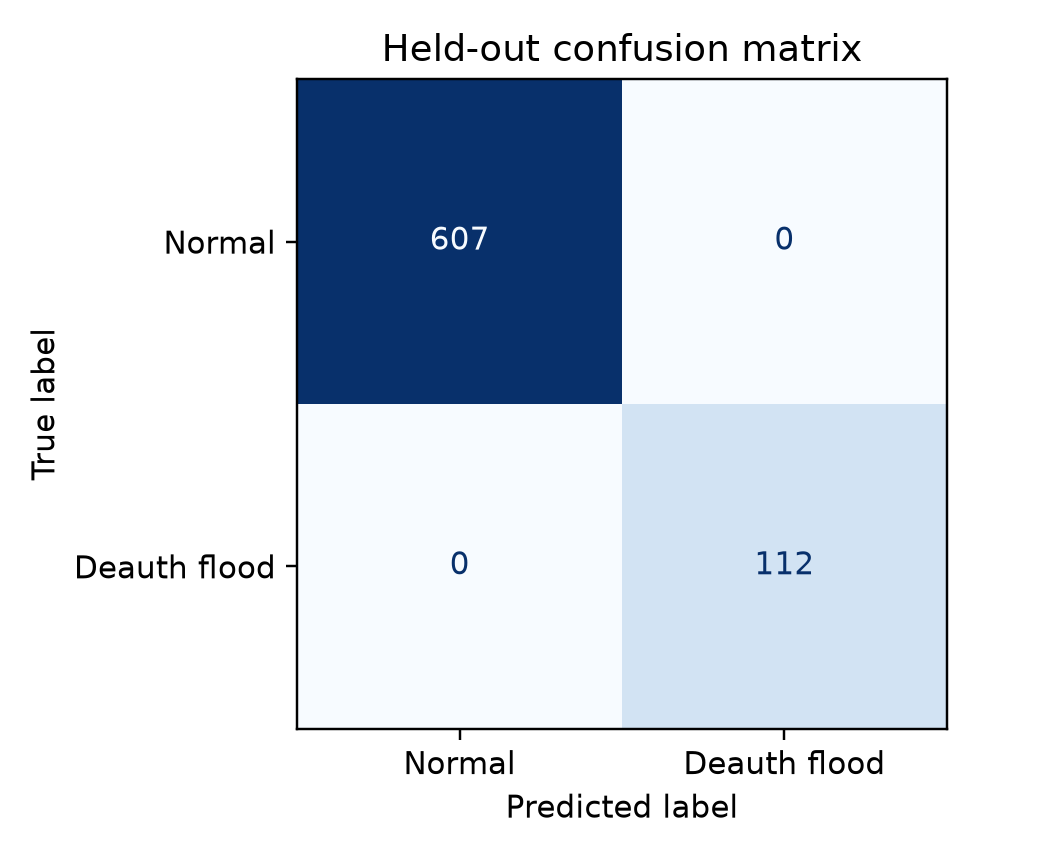
\includegraphics[width=\linewidth]{../results/confusion_matrix_random_forest.png}\\[-1mm]
{\fontsize{16}{19}\selectfont Confusion matrix on held-out later traffic.}
\end{center}

\begin{center}
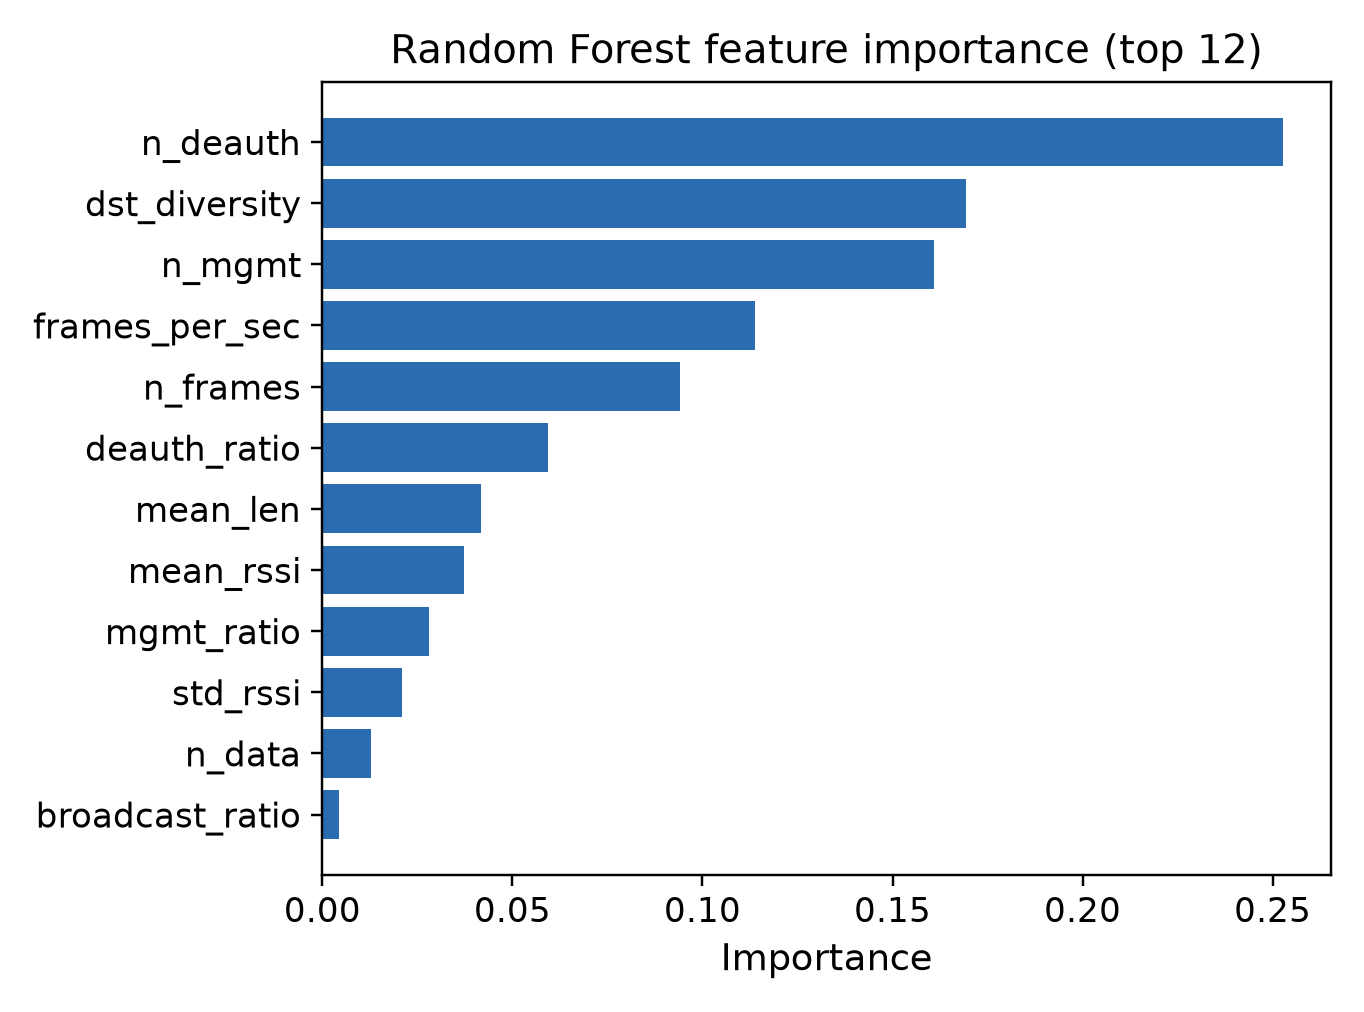
\includegraphics[width=\linewidth]{../results/feature_importance.png}\\[-1mm]
{\fontsize{16}{19}\selectfont Random Forest feature importance (top 12).}
\end{center}

\columnbreak

\heading{Detection demo}
60 s normal excerpt: \textbf{no alerts}.

60 s attack excerpt:
\begin{tcolorbox}[colback=black!92,coltext=white,boxrule=0pt,arc=1mm,
  left=3mm,right=3mm,top=2mm,bottom=2mm]
{\ttfamily\fontsize{14}{17}\selectfont
[ALERT 1] 07:34:12 to 07:35:07\\
MAC 02:00:00:00:00:72\\
deauth=215/s  RSSI=-29 dBm  score=1.00\\[1mm]
[ALERT 2] 07:34:12 to 07:35:07\\
MAC 02:00:00:00:00:cb\\
deauth=1289/s  RSSI=-32 dBm  score=1.00}
\end{tcolorbox}

On the full 15-minute capture the detector found the two sustained floods.
Two short low-rate exchanges (3 to 16/s) were filtered by the 20/s rule.

\heading{Limitations}
\begin{itemize}[leftmargin=5mm,itemsep=1mm,topsep=1mm]
  \item One capture, one testbed, so 100\% is optimistic.
  \item 1-second windows, and only deauth floods are modelled.
  \item MAC spoofing makes the source in the alert unreliable.
  \item No live monitor-mode test because the VM has no adapter. The PCAP replay path is used.
  \item Two low-rate episodes are false positives at window level, but the rate rule suppresses them.
\end{itemize}

\heading{What I would improve}
\begin{itemize}[leftmargin=5mm,itemsep=1mm,topsep=1mm]
  \item Test on AWID3 and new captures from different networks.
  \item Add disassociation floods, beacon floods and evil twin detection.
  \item Try sliding windows and online learning for concept drift.
  \item Test evasion with low-rate, bursty or spoofed-source attacks.
  \item Add a live dashboard and maybe AP integration.
\end{itemize}

\heading{AI use}
I used OpenCode with a DeepSeek model to help me find and download the public
dataset, set up the Python pipeline, debug the tshark extraction and draft the
poster text. I checked the dataset and code, ran the training and evaluation,
and confirmed that no MAC address or timestamp is used as a feature. All
reported numbers come from the included scripts.

\heading{Reproduce}
\begin{tcolorbox}[colback=lightgrey,colframe=lightgrey,boxrule=0pt,arc=1mm,
  left=3mm,right=3mm,top=2mm,bottom=2mm]
{\ttfamily\fontsize{15}{18}\selectfont
python prepare\_data.py\\
python train.py\\
python detect.py --pcap data/demo\_attack.pcap}
\end{tcolorbox}

\vspace{2mm}
{\color{navy}\rule{\linewidth}{0.8mm}}\\[1mm]
{\fontsize{15}{18}\selectfont Code and results: local submission.\\
Dataset DOI: 10.17632/cxx5t5nw7z.3. Python, tshark, scikit-learn.}

\end{multicols}

\vfill

\begin{tcolorbox}[colback=navy,coltext=white,boxrule=0pt,arc=2mm,
  left=8mm,right=8mm,top=4mm,bottom=4mm]
\begin{minipage}[c]{0.70\linewidth}
{\color{amber}\fontsize{24}{28}\selectfont\bfseries Bottom line}\\[1mm]
{\fontsize{20}{24}\selectfont A Random Forest on per-MAC, per-second features
detects deauthentication floods with 100\% accuracy on held-out traffic and
gives a MAC-level alert.}
\end{minipage}\hfill
\begin{minipage}[c]{0.26\linewidth}
\centering
{\color{amber}\fontsize{20}{24}\selectfont\bfseries Key numbers}\\[1mm]
{\fontsize{18}{22}\selectfont 722,606 frames\\207,222 deauth\\2,692 windows\\100\% accuracy}
\end{minipage}
\end{tcolorbox}

\end{document}
